\documentclass[a4paper,t,xcolor=pst,dvips,colortheme]{beamer}

\usepackage{beamerthemesplit}
\usepackage[utf8]{inputenc}
\usepackage[spanish]{babel}
\usepackage{graphicx}
\usepackage{pstricks} % PSTricks package
\usepackage{setspace}
\usepackage{multirow}
\usepackage{listings}
\usepackage{pgfpages}
\usepackage{hyperref}
\usepackage{etoolbox}
% \usepackage{epstopdf}

\makeatletter
\patchcmd{\beamer@sectionintoc}{\vskip1.5em}{\vskip0.5em}{}{}
\makeatother

\setbeamercovered{dynamic}
\setcounter{tocdepth}{3}
\setbeamercolor{frametitle}{fg=black,bg=white}
\setbeamercolor{section in toc shaded}{fg=black}
\setbeamercolor{section in toc}{fg=red}
\setbeamercolor{subsection in toc shaded}{fg=black}
\setbeamercolor{subsection in toc}{fg=red}
\setbeamerfont{section in toc}{size=\small}
\setbeamerfont{subsection in toc}{size=\small}
\setbeamertemplate{section in toc shaded}[default][99]
\setbeamertemplate{subsection in toc shaded}[default][99]

\AtBeginSection[]
{\begin{frame}[c]
  \frametitle{Índice}
	\tableofcontents[currentsection,
        sectionstyle=show/shaded,
        subsectionstyle=hide]
\end{frame}}

\AtBeginSubsection[]
{\begin{frame}[c]
	\frametitle{Índice}
	\tableofcontents[
  		currentsection,
  		sectionstyle=shaded/shaded,
  		currentsubsection,
  		subsectionstyle=show/shaded/hide
		]
\end{frame}}

\setbeamercolor{frametitle}{fg=black,bg=white}

\setbeamertemplate{frametitle}{
	\begin{centering}
		\insertframetitle
		\par
	\end{centering}
}

\usetheme[secheader]{Boadilla}


\title[Computadores y Juegos]{¿Cómo juega un computador al ajedrez \\ y por qué no puedo ganarle?}

\author[Pablo Sánchez]{\alert{Pablo Sánchez}}

\institute[I2E]{
		   Dpto. Ingenier{\'i}a Inform{\'a}tica y Electr{\'o}nica \\
		   Universidad de Cantabria \\
		   Santander (Cantabria, España) \\
		   p.sanchez@unican.es
}

\date{}

\begin{document}

\begin{frame}[c]
	\titlepage
	\begin{columns}
		\column{0.50\linewidth}
			\centering
    		
\includegraphics[width=.28\textwidth,keepaspectratio=true]{images/istr.eps}
		\column{0.50\linewidth}
			\centering
			
\includegraphics[width=.25\textwidth,keepaspectratio=true]{images/uc.eps}
	\end{columns}
\end{frame}

\section{Introducción}

\subsection{Motivación}

\begin{frame}[t]
    \only<1|handout:0>{
        \rput[lt](0,-1){
            
\includegraphics[width=\linewidth]{images/intro/dragon00.eps}
        }
    }
    \only<2|handout:0>{
        \rput[lt](0,-1){
            
\includegraphics[width=\linewidth]{images/intro/dragon01.eps}
        }
    }
    \only<3|handout:0>{
        \rput[lt](0,-1){
            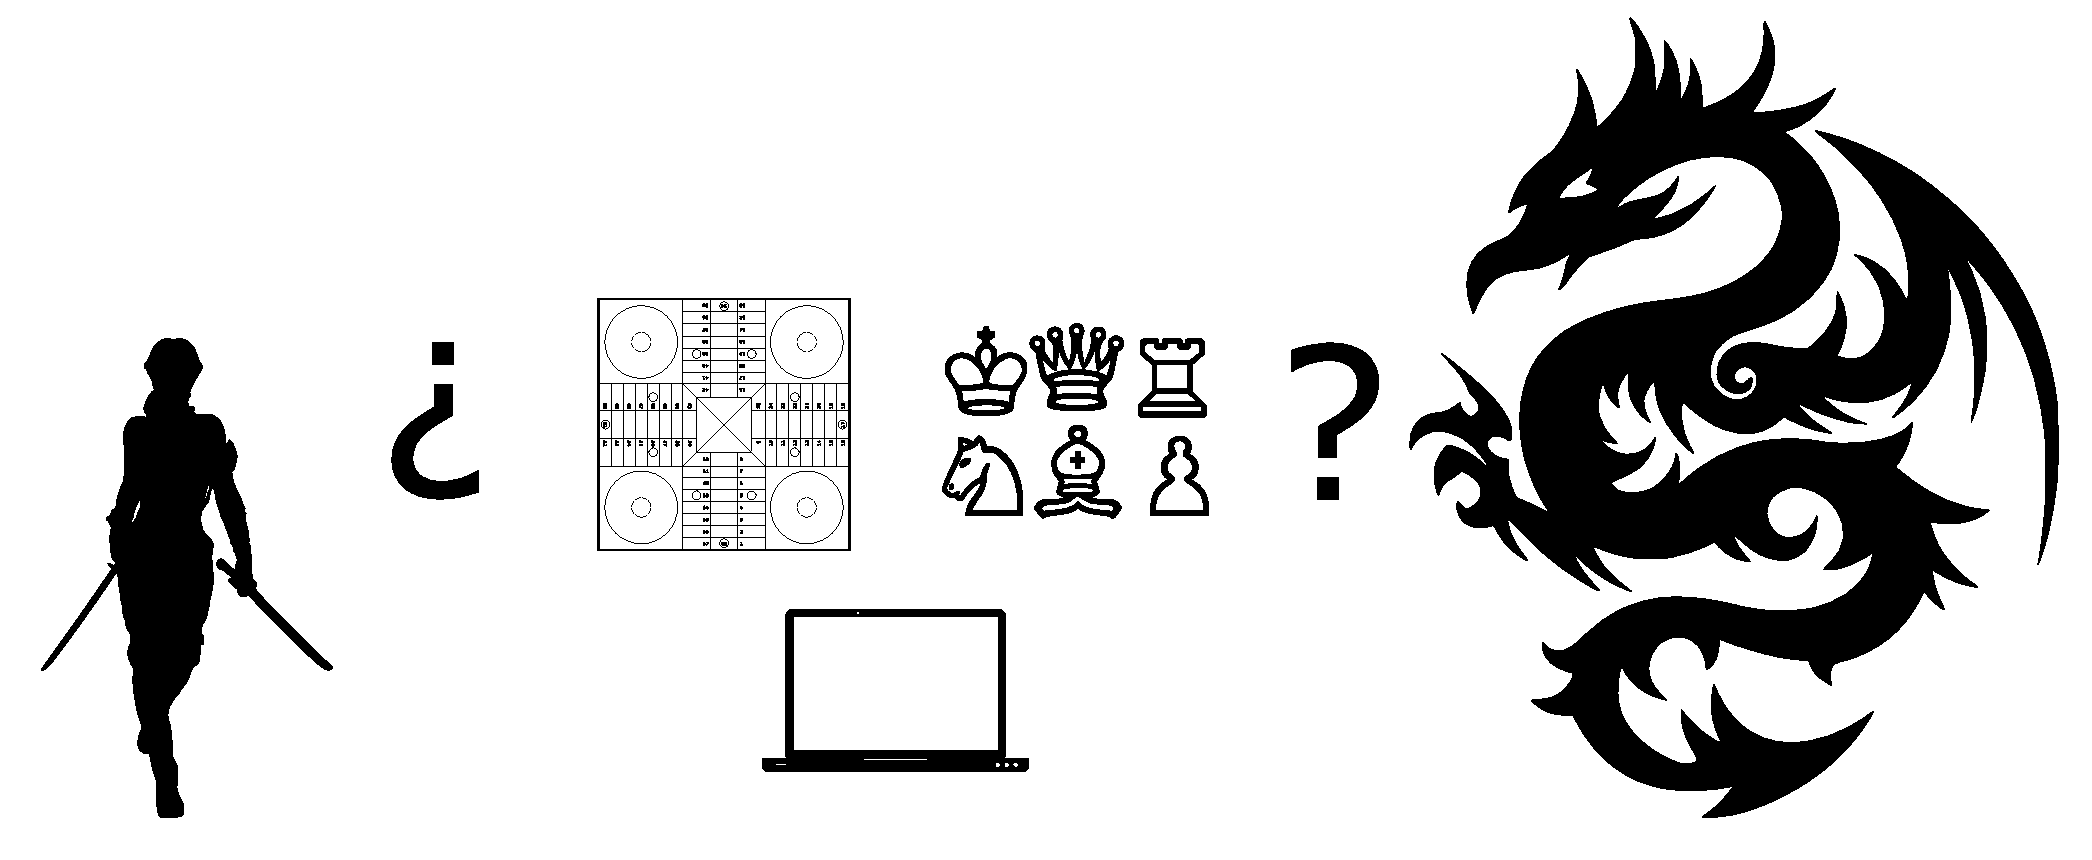
\includegraphics[width=\linewidth]{images/intro/dragon02.eps}
        }
    }
    \only<4|handout:0>{
        \rput[lt](0,-1){
            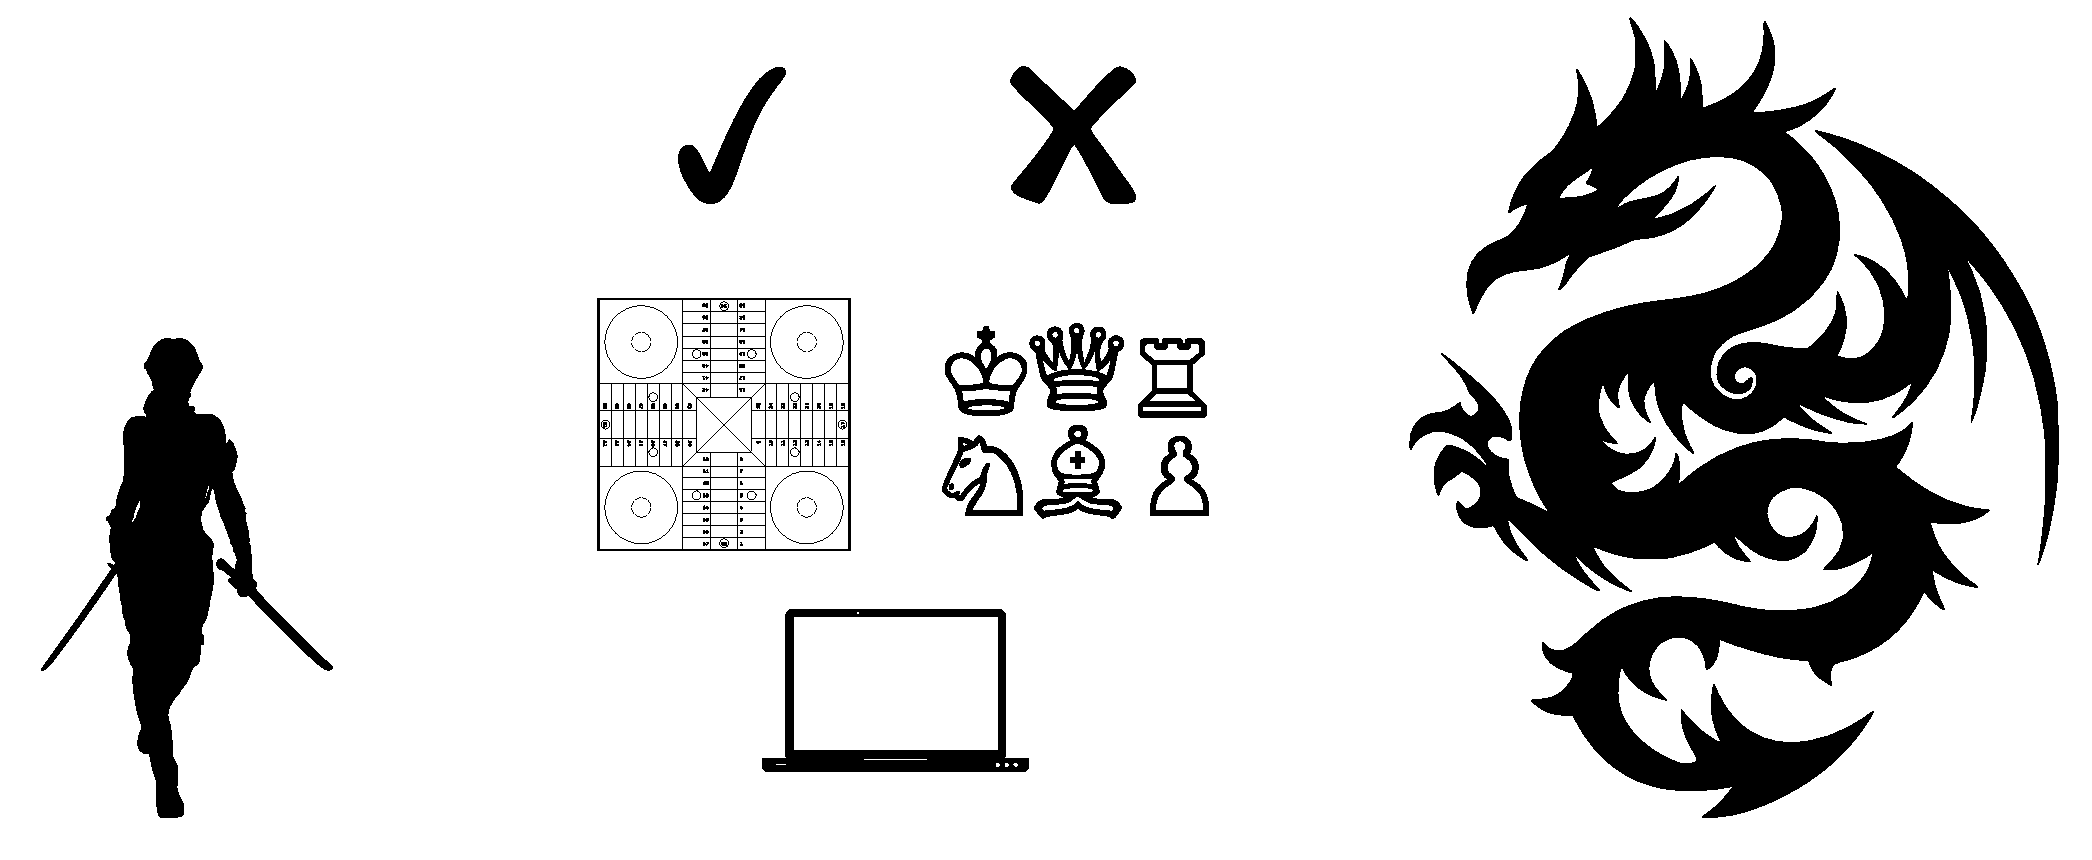
\includegraphics[width=\linewidth]{images/intro/dragon03.eps}
        }
    }
\end{frame}

\subsection{¿Qué Sabe Hacer un Computador?}

\begin{frame}[c]
    \frametitle{¿Qué Sabe Hacer un Computador?}    
    \begin{enumerate}[<+->]
        \item Sumas y restas. 
        \item (Multiplicaciones y Divisiones).
        \item Comparar números por igualdad.
        \item Comparar números por desigualdad.
        \item Decidir el siguiente paso a ejecutar en función de una comparación.
        \item Leer y escribir números en memoria.
    \end{enumerate}
\end{frame}

\begin{frame}[c]
    \frametitle{¿Qué Sabe Hacer un Computador?}
    \begin{center}
       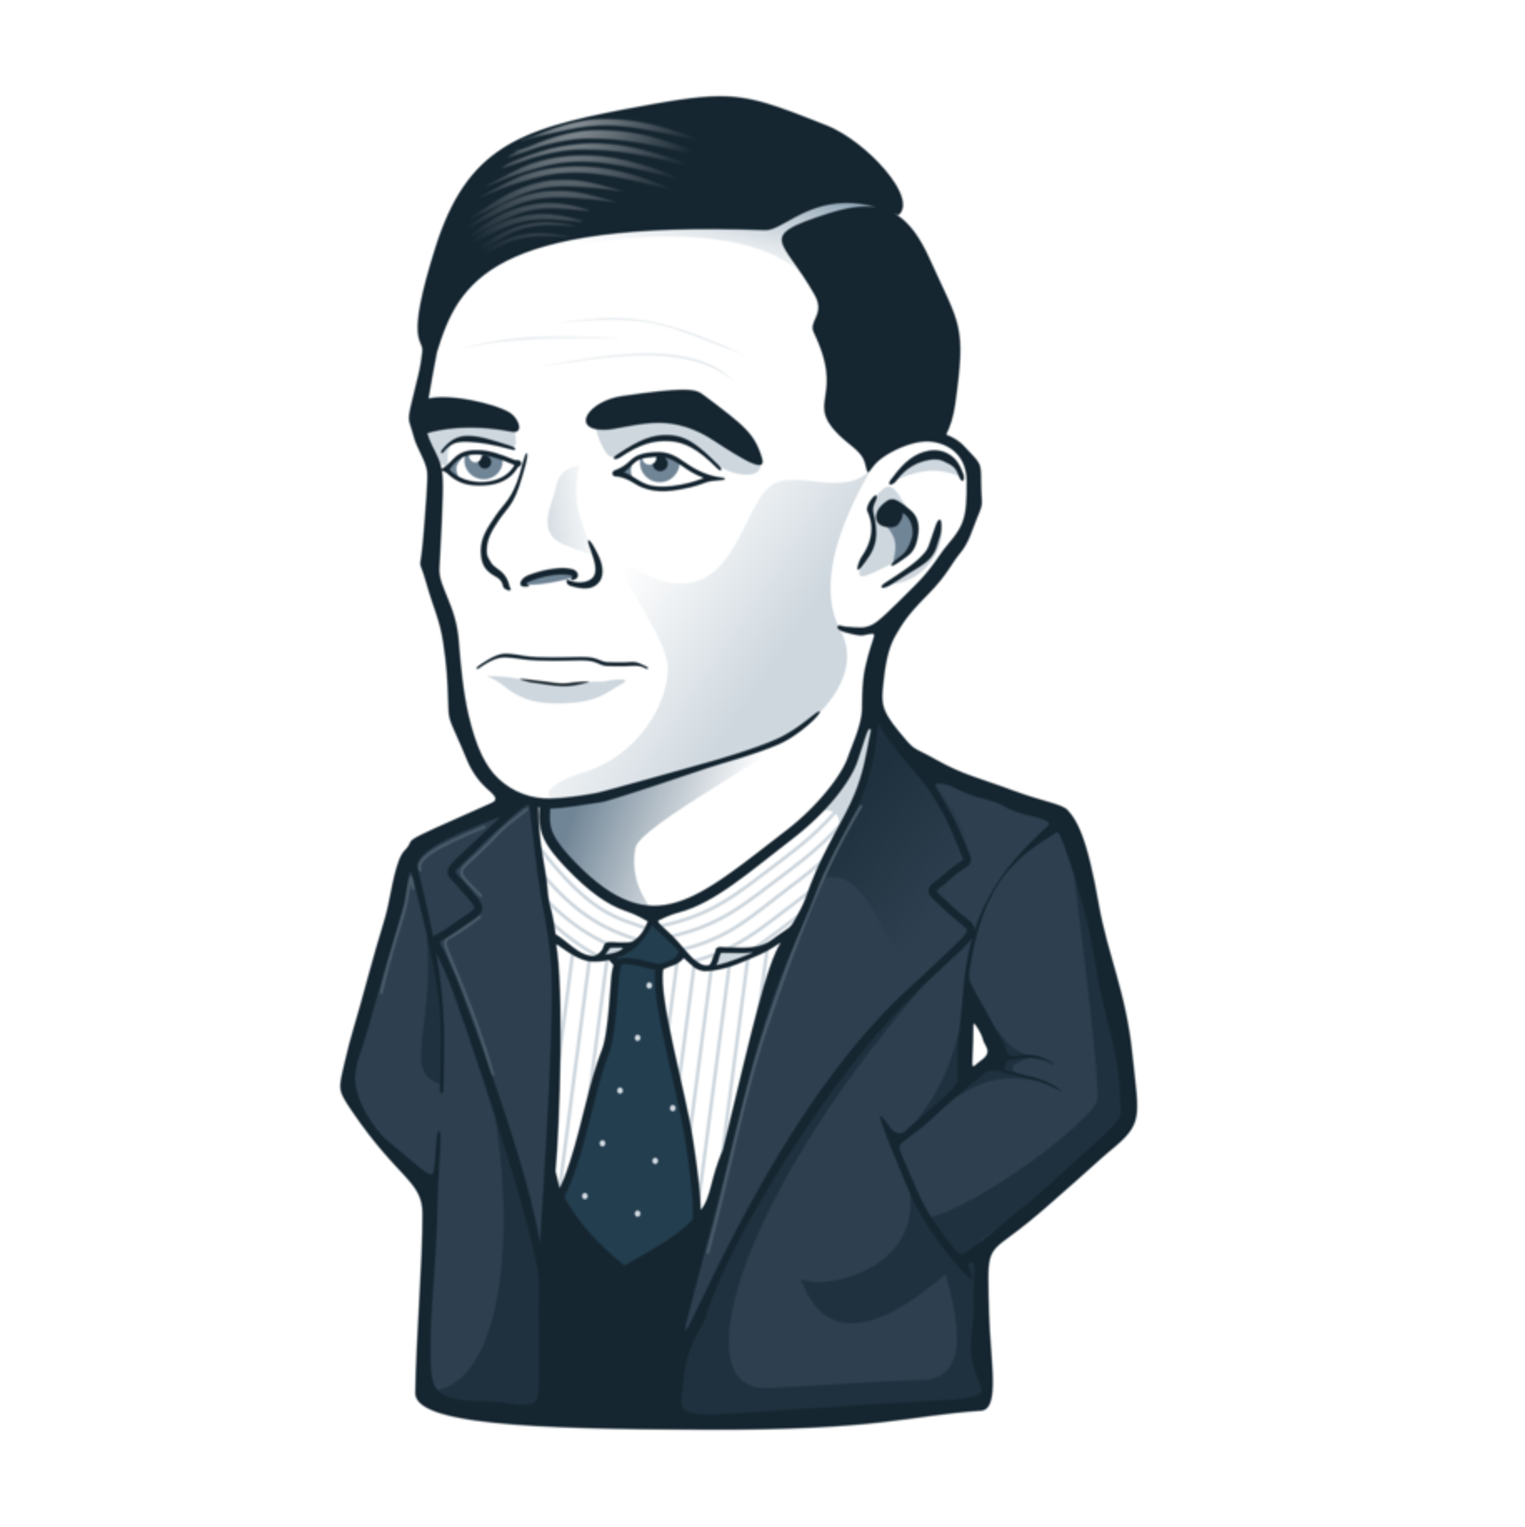
\includegraphics[width=0.5\linewidth]{images/intro/alanTuring.eps} \\ 
        \textbf{Alan Turing}
    \end{center}
    
    %% Imagen de Alan Turing

    %% 1952, Alan Turing procesado por delito de homosexualidad.
    %% Acepta castración química
    %% 1954, muere tras ingerir una manzana envenada con cianuro (suicido, asesinato, despiste)
    %% 2009, Gordon Brown pide públicamente disculpas
    %% 2012, David Cameron deniega el indulto.
    %% 2013, Indulto real 
    
    %% https://elpais.com/sociedad/2013/11/13/actualidad/1384332286_406469.html
    %% Hidrogenesse, Un dígito binario dudoso. Recital para Alan Turing
\end{frame}

\begin{frame}[c]
    \frametitle{¿Qué Sabe Hacer un Computador?}
    \begin{enumerate}[<+->]
        \item Un computador sólo hace operaciones básicas.
        \item Pero hace un billón (europeo) de operaciones básicas por segundo.
        \item A un computador se le da bien \emph{buscar una aguja en un pajar}.
        \item Un computador no siente cansancio o frustración.
        \item Un computador consume energía y produce CO$_{2}$.
    \end{enumerate}
\end{frame}

\section{Juegos Básicos: Algoritmo Minimax}

\begin{frame}[c]
    \frametitle{Algoritmo Minimax}
    \begin{enumerate}[<+->]
        \item Represento el juego como un conjunto de números.
        \item Especifico cómo realizar movimientos válidos como una serie de operaciones básicas.
        \item Especifico cómo decidir si el juego ha terminado. 
        \item Especifico cómo decidir cuán buena es la victoria (si hay diferencias).
    \end{enumerate}
\end{frame}




\section{Backtracking y Ramificación y Poda}

\section{Redes Neuronales: Jugando Parchís}

\end{document} 